%
% lineariaet.tex
%
% (c) 2018 Prof Dr Andreas Müller, Hochschule Rapperswil
%
\documentclass[tikz]{standalone}
\usepackage{times}
\usepackage{amsmath}
\usepackage{txfonts}
\usepackage[utf8]{inputenc}
\usepackage{graphics}
\usetikzlibrary{arrows,intersections,math}
\begin{document}

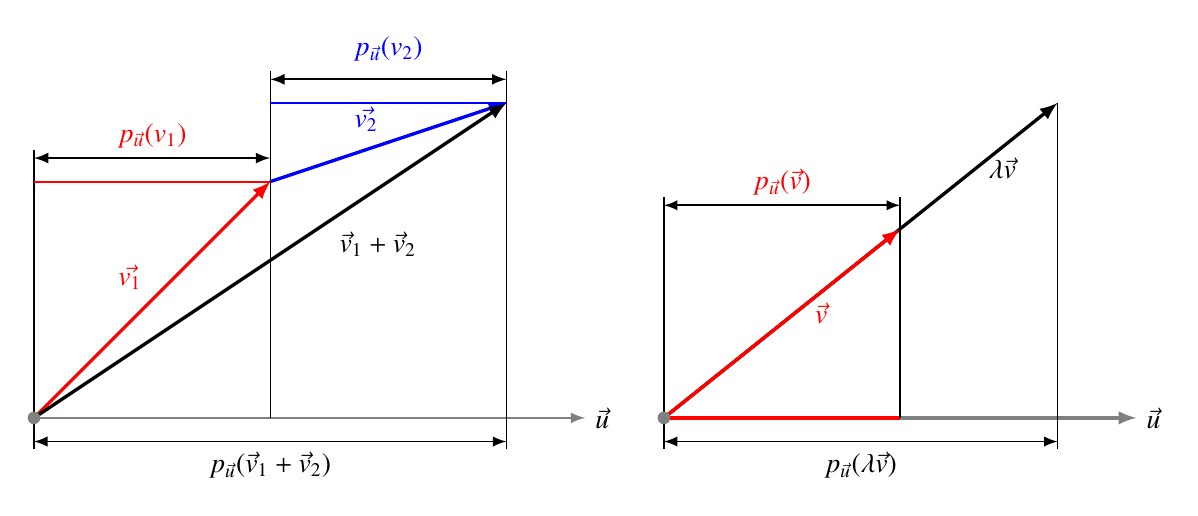
\begin{tikzpicture}[>=latex,thick]

% Teilbild links: Linearitaet der Summe
\begin{scope}

% Vektor u
\draw[->,color=gray] (0,0)--(7,0);
\node at (7,0) [right] {$\vec{u}$};

% Vektoren v1 und v2
\draw[->,color=red,line width=1.2pt] (0,0)--(3,3);
\node[color=red] at (1.5,1.5) [above left] {$\vec{v_1}$};

\draw[->,color=blue,line width=1.2pt] (3,3)--(6,4);
\node[color=blue] at (4.5,3.5) [above left] {$\vec{v_2}$};

% Summenvektor
\draw[->,line width=1.2pt] (0,0)--(6,4);
\node at (3.75,2.5) [below right] {$\vec{v}_1+\vec{v}_2$};

% Projektionen
\draw[line width=0.5pt] (0,-0.4)--(0,3.4);
\draw[line width=0.5pt] (3,0)--(3,4.4);
\draw[line width=0.5pt] (6,-0.4)--(6,4.4);

\draw[color=red,line width=0.7pt] (0,3)--(3,3);
\node[color=red] at (1.5,3.3) [above] {$p_{\vec{u}}(v_1)$};
\draw[<->] (0,3.3)--(3,3.3);

\draw[color=blue,line width=0.7pt] (3,4)--(6,4);
\node[color=blue] at (4.5,4.4) [above] {$p_{\vec{u}}(v_2)$};
\draw[<->] (3,4.3)--(6,4.3);

% Projektion der Summe
\draw[<->,line width=0.7pt] (0,-0.3)--(6,-0.3);
\node at (3,-0.3) [below] {$p_{\vec{u}}(\vec{v}_1+\vec{v}_2)$};

% Nullpunkt
\fill[color=gray] (0,0) circle[radius=0.08];

\end{scope}

% Teilbild rechts: Linearitaet der Multiplikation mit Skalaren
\begin{scope}[xshift=8cm]

% Vektor u
\draw[->,color=gray,line width=1.2pt] (0,0)--(6,0);
\node at (6,0) [right] {$\vec{u}$};

% Vektor \lambda v
\draw[->,line width=1.2pt] (0,0)--(5,4);
\node at (4.3,{4.3*0.8}) [below] {$\lambda\vec{v}$};

% Vektor v
\draw[->,line width=1.25pt,color=red] (0,0)--(3,2.4);
\draw[color=red,line width=1.2pt] (0,{0*2.4})--(3,{0*2.4});
\node[color=red] at (2,1.6) [below] {$\vec{v}$};

% Bemassung
\draw[<->,line width=0.7pt] (0,2.7)--(3,2.7);
\node[color=red] at (1.5,2.7) [above] {$p_{\vec{u}}(\vec{v})$};

\draw[<->,line width=0.7pt] (0,-0.3)--(5,-0.3);
\node at (2.5,-0.3) [below] {$p_{\vec{u}}(\lambda\vec{v})$};

% Projektionslinien
\draw[line width=0.5pt] (0,2.8)--(0,-0.4);
\draw[line width=0.5pt] (3,2.8)--(3,0);
\draw[line width=0.5pt] (5,4)--(5,-0.4);

\fill[color=gray] (0,0) circle[radius=0.08];

\end{scope}

\end{tikzpicture}

\end{document}

